\section{Application Case Study: massive MIMO 5G Evaluation}
\label{sec:exp2-nr-energy}

Having successfully verified the computational efficiency and scalability of our embedded simulation framework, we now demonstrate its practical utility through a realistic 3GPP~NR deployment case study \cite{5glena,tr38901}.
This section showcases how the integrated Sionna~RT backend allows researchers to evaluate end-to-end 5G massive MIMO networks. We assess critical application-level KPIs (throughput, packet loss, delay, jitter), propagation-level KPIs (path loss, path delay, CQI, MCS), and overall energy consumption. To provide a comprehensive evaluation, we simulate three distinct radio environments—free space, urban macro, and urban micro—using gNB antenna array sizes ranging from $2\times2$ to $8\times8$, under varying traffic loads.

\subsection{Experiment Configuration}
\label{subsec:exp2-setup}

In each simulation run, one gNB and 20 UEs are used.
The UE count is fixed to 20 to keep per-step GPU memory and simulation wall-clock time within practical bounds on the evaluation hardware; scaling to denser deployments is outside the scope of this work.
The gNB antenna array is varied over $2\times2$, $4\times4$, and $8\times8$; each UE uses a fixed $2\times2$ array.
The simulations are tested in three different radio environments:
\begin{itemize}
    \item \textbf{free space}: $2$ GHz carrier, $35$ m gNB height, and UE
          distances from $50$ m to $1000$ m;
    \item \textbf{urban macro}: $3.5$ GHz carrier, $25$ m gNB height, and UE
          distances from $35$ m to $500$ m;
    \item \textbf{urban micro}: $28$ GHz carrier, $10$ m gNB height, and UE
          distances from $10$ m to $200$ m.
\end{itemize}
The carrier frequencies, antenna heights, and UE distance ranges are aligned with the 3GPP TR 38.901 reference deployment configurations \cite{tr38901}.
The 2~GHz carrier for the free-space baseline corresponds to the FR1 sub-3~GHz band; the 3.5~GHz urban macro carrier matches the primary 5G~NR band (n78, FR1); and the 28~GHz urban micro carrier represents the FR2 mmWave band (n257/n261).
The gNB heights of 25~m (urban macro) and 10~m (urban micro) follow the TR~38.901 UMa and UMi reference values respectively, while the 35~m free-space height is consistent with rural macro conventions.
The UE distance ranges are chosen to cover the minimum coupling distance and approximate cell radius defined for each scenario in TR~38.901 Table~7.2-1.
The single-cell, 20-UE configuration is consistent with the single-sector system-level evaluation methodology of TR~38.901 Table~A.1.
The free-space scenario is the baseline, the urban macro scenario represents a sub-6~GHz deployment, and the urban micro scenario represents the most demanding physical setting as it combines a mmWave carrier with geometry-sensitive, short-range links.
The 3D visualizations of these three environments are shown in Figure~\ref{fig:scenarios}.

\begin{figure}[t]
    \centering
    \subfloat[Free space.]{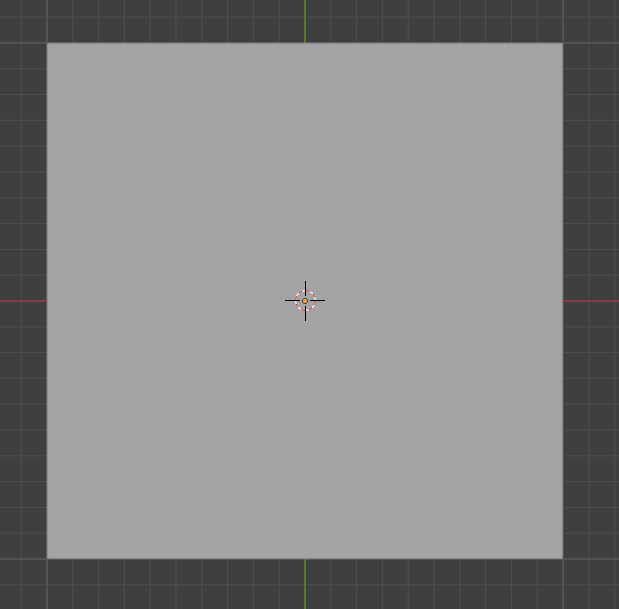
\includegraphics[width=0.32\linewidth]{images/free_space.png}\label{fig:scenario_free_space}}
    \hfill
    \subfloat[Urban macro.]{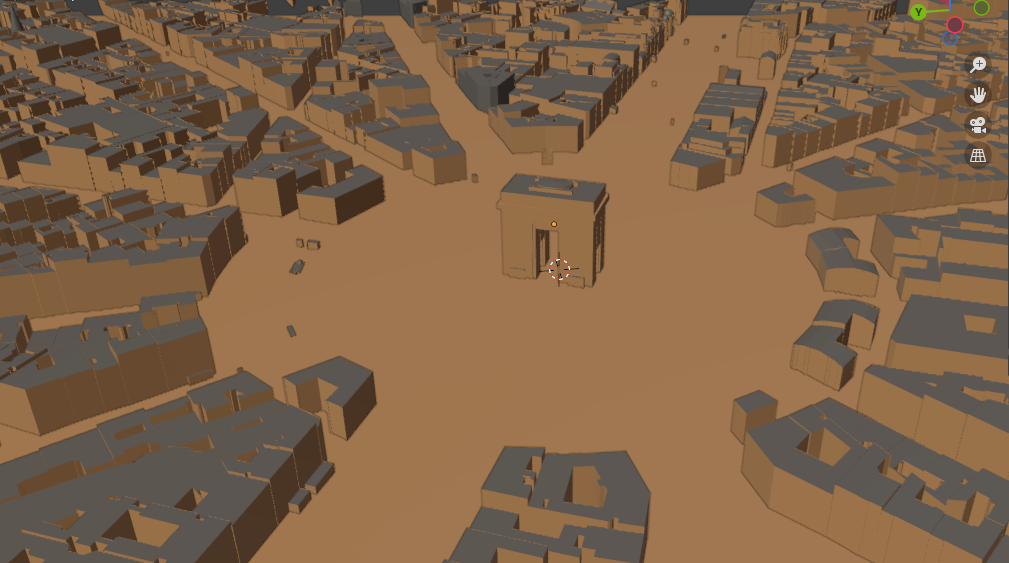
\includegraphics[width=0.32\linewidth]{images/urban_macro.png}\label{fig:scenario_urban_macro}}
    \hfill
    \subfloat[Urban micro.]{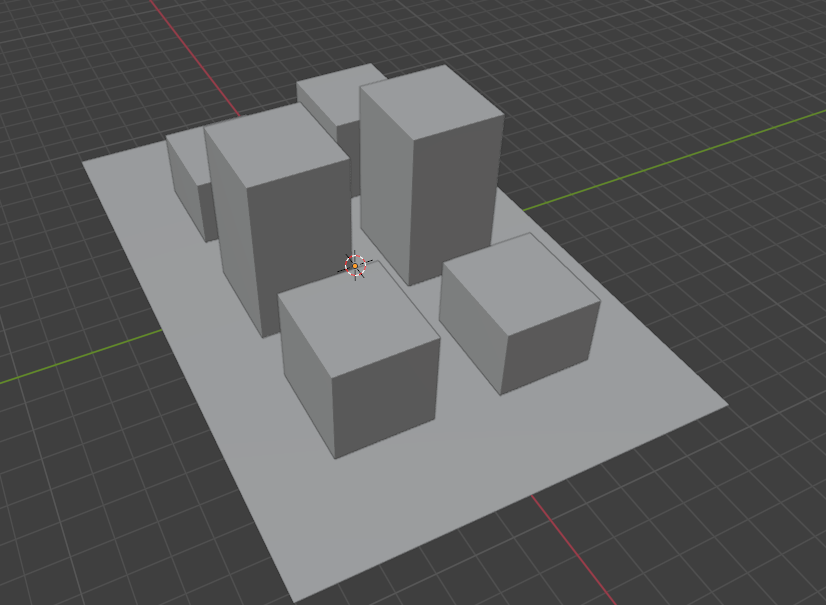
\includegraphics[width=0.32\linewidth]{images/urban_micro.png}\label{fig:scenario_urban_micro}}
    \caption{The three simulated radio environments.}
    \label{fig:scenarios}
\end{figure}

For scheduling UEs, a TDMA proportional fair scheduler, and full-buffer TDD slots are used.
On top of the realistic wireless channel model, different applications with different traffic loads are tested.
The traffic profile includes video, voice over IP (VoIP), social media, gaming, and FTP.
The per-application UE distribution — 12 (60\%), 2 (10\%), 2 (10\%), 1 (5\%), and 3 (15\%) for video, VoIP, social media, gaming, and FTP respectively — follows the traffic mix proportions reported in \cite{ericsson_mobility}, and is applied identically for both DL and UL.
The data rate for each application according to load levels are summarized in Table \ref{tab:exp2-offered-load}.

\begin{table*}[t]
    \centering
    \caption{Application data rate by application and load.}
    \label{tab:exp2-offered-load}
    \begin{tabular}{lrrrrrrr}
        \hline
        Application                & Flows                    & \multicolumn{2}{c}{Low} &
        \multicolumn{2}{c}{Medium} & \multicolumn{2}{c}{High}                                                                                       \\
        \cline{3-8}
                                   &                          & DL (Mbps)               & UL (Mbps) & DL (Mbps) & UL (Mbps) & DL (Mbps) & UL (Mbps) \\
        \hline
        Video                      & 12 DL / 12 UL            & 24.000                  & 0.300     & 96.000    & 1.200     & 300.000   & 3.750     \\
        VoIP                       & 2 DL / 2 UL              & 0.128                   & 0.032     & 0.256     & 0.064     & 2.000     & 0.500     \\
        Social                     & 2 DL / 2 UL              & 1.000                   & 0.050     & 10.000    & 0.500     & 40.000    & 2.000     \\
        Gaming                     & 1 DL / 1 UL              & 0.100                   & 0.025     & 1.000     & 0.250     & 10.000    & 2.500     \\
        FTP                        & 3 DL / 3 UL              & 3.000                   & 0.150     & 30.000    & 1.500     & 150.000   & 7.500     \\
        \hline
        Total                      & 20 DL / 20 UL            & 28.228                  & 0.557     & 137.256   & 3.514     & 502.000   & 16.250    \\
        \hline
    \end{tabular}
\end{table*}


\subsection{Free-Space Scenario}
\label{subsec:exp2-free-space}

The free-space scenario serves as the baseline because it has no building blockage; distance is the sole large-scale factor.
UEs are distributed up to $1000$~m from the gNB, so the scenario combines strong near-field links with very weak cell-edge links.

\subsubsection{Application-related Metrics}
\label{subsubsec:exp2-free-space-flow}

Figure~\ref{fig:exp2-free-space-flow} shows per-application throughput, packet loss, delay, and jitter for both directions and all antenna configurations.
The stochastic ns-3 model outperforms Sionna~RT in average downlink throughput: at $8\times8$, ns-3 delivers $4.85$~Mbit/s ($21.6\%$ loss) versus $3.77$~Mbit/s ($26.6\%$ loss) for Sionna~RT, with the same ordering at $2\times2$.
The gap reflects the large cell radius: UEs at the cell edge experience greater path loss under ray tracing than the stochastic model predicts.
Array scaling yields only marginal throughput gain in both simulators because the bottleneck is cell-edge path loss, not beamforming resolution.

\begin{figure*}[t]
    \centering
    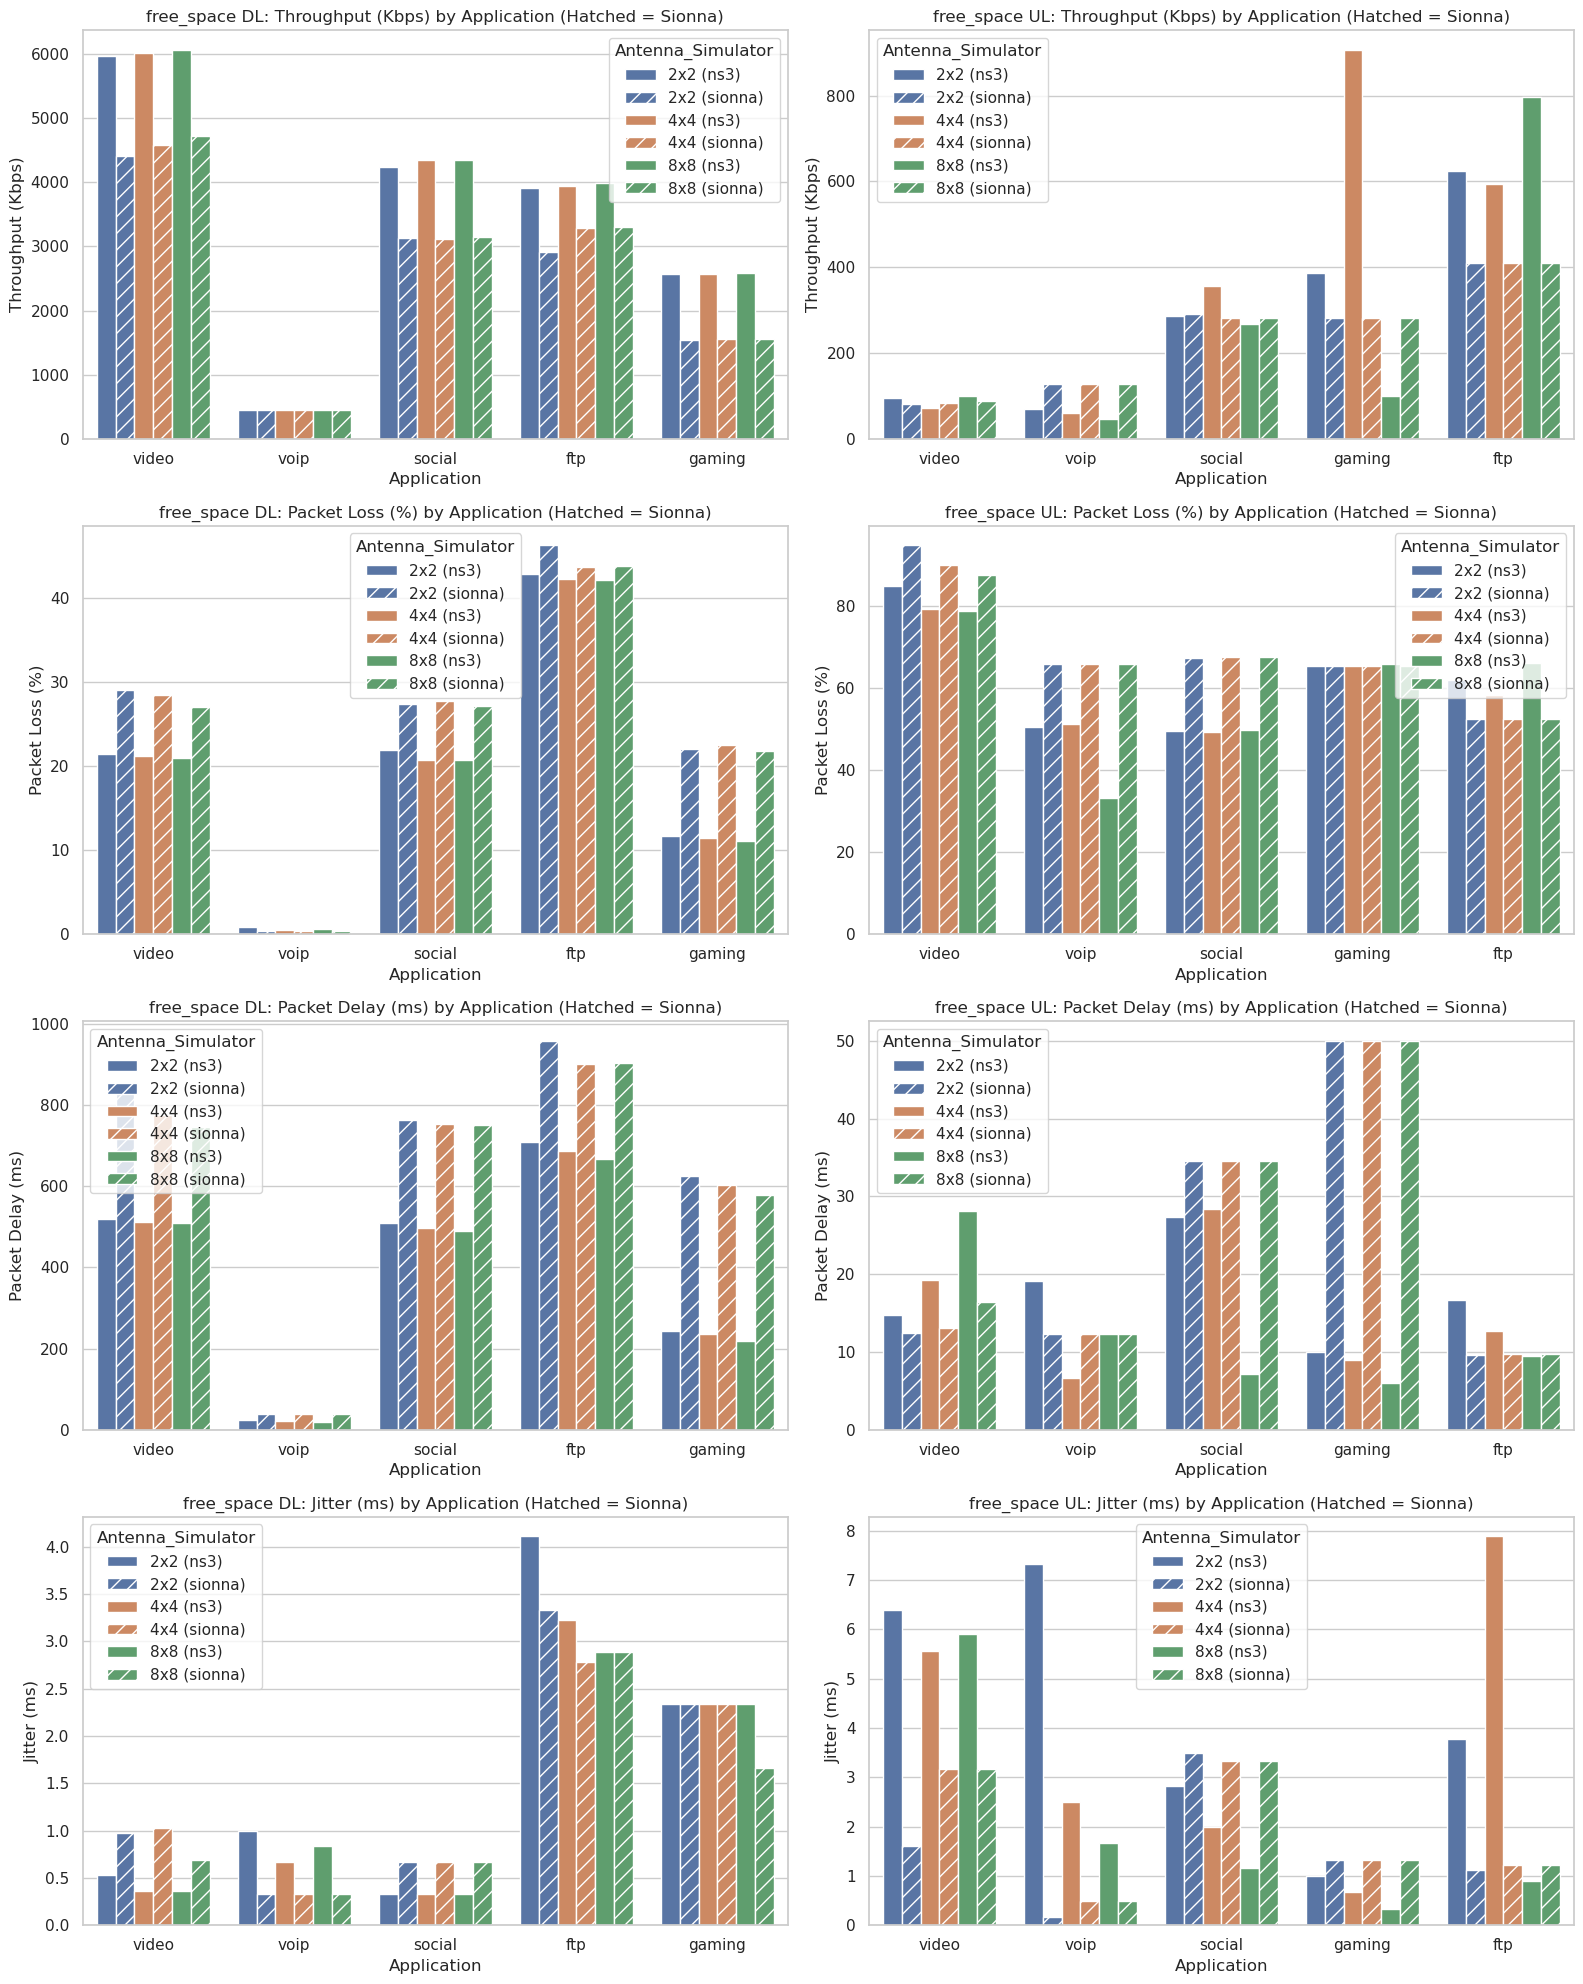
\includegraphics[width=\textwidth]{images/free_space_flow_metrics.png}
    \caption{Free-space application-level throughput and packet loss by application, direction, and gNB array size. Solid bars: ns-3; hatched bars: Sionna~RT.}
    \label{fig:exp2-free-space-flow}
\end{figure*}

\subsubsection{Propagation-related Metrics}
\label{subsubsec:exp2-free-space-propagation}

Average path loss is $94.2$~dB and estimated receive power is $-48.2$~dBm for both channel models (Fig.~\ref{fig:exp2-channel-quality}).
The ns-3 model reports a mean path delay of $3059$~ns while Sionna~RT reports $2237$~ns; both are consistent with radio path lengths of hundreds of metres.
CQI and MCS improve monotonically with array size in both simulators.
At $8\times8$, ns-3 reaches mean CQI~$15$ and MCS~$27$; Sionna~RT reaches CQI~$14.79$ and MCS~$26.59$.
The gap is small in free space because most links are near-line-of-sight; array gain raises channel quality but cannot overcome path loss for the most remote UEs.

\subsubsection{Energy Consumption-related Metrics}
\label{subsubsec:exp2-free-space-energy}

gNB power consumption increases with array size in both simulators (Fig.~\ref{fig:exp2-gnb-power}).
In ns-3, the gNB consumes $31.16$~W ($2\times2$), $64.58$~W ($4\times4$), and $199.39$~W ($8\times8$); Sionna~RT reports $30.08$~W, $59.08$~W, and $173.50$~W respectively.
UE power is similar across all configurations because the UE array is fixed at $2\times2$.
The throughput-per-watt trade-off is poor for larger arrays in this scenario: $8\times8$ consumes roughly six times the gNB power of $2\times2$ while delivering only marginal throughput gains.
Array gain cannot offset the scheduling pressure of serving many long-distance UEs under high traffic load.


\subsection{Urban Macro Scenario}
\label{subsec:exp2-urban-macro}

The urban macro scenarios is based on the Charles de Gaulle Etoile in Paris, which is a dense urban environment with tall buildings and many obstacles.
The gNB is placed at the top of the Arc de Triomphe at a height of $25$ m and UEs are distributed in a circle of radius $500$ m around the gNB.
The antennas are configured to use the $3.5$ GHz carrier frequency, which is in the sub 6-Hz range.
This scenario is one of the challenging scenario for 6G network deployments due to the high density of buildings and obstacles.

\subsubsection{Application-related Metrics}
\label{subsubsec:exp2-urban-macro-flow}

Figure \ref{fig:exp2-urban-macro-flow} illustrates the application-related metrics for the urban macro scenario, comparing ns-3 (solid bars) and Sionna RT (hatched bars) across various antenna configurations.
Among the traffic types, data-intensive applications such as FTP and video streaming achieve the highest throughput in both simulators.
For FTP, ns-3 outperforms Sionna RT at the $2 \times 2$ configuration where ns-3 achieve roughly $16.8$ Mbps whereas Sionna RT achieve $15.2$ Mbps.
But as the gNB array size increase to $4 \times 4$ and $8 \times 8$, Sionna RT perform better than ns-3 and achieve nearly $19.5$ Mbps whereas ns-3 achieve $18.5$ Mbps.
The statistical ns-3 approach performs well generally but Sionna RT approach performs better at larger array size as it can better leverage massive MIMO spatial multiplexing by capturing multipath components such as reflections and diffractions from the buildings and environment.
In contrast, for video streaming application, ns-3 consistently achieve higher than Sionna RT across all antenna configurations.

For Sionna RT, higher packet loss for video traffic is observed in downlink which values are $9.5\%$, $7.6\%$ and $4.6\%$ respectively for $2 \times 2$, $4 \times 4$ and $8 \times 8$ antenna configurations.
Ns-3 performs better than Sionna RT for video traffic and for FTP traffic under $2 \times 2$ configuration, however, Sionna RT outperforms ns-3 for FTP traffic under $4 \times 4$ and $8 \times 8$ configurations.
Overall, increasing the antenna array size significantly reduce packet loss for most of the applications in both simulators.
In the uplink, the packet loss for all most all of the applications are very high for both simulators, ranging from $15\%$ for VoIP to nearly $100\%$ for gaming and social applications in Sionna RT.
This reflects the impact of harsh environment conditions on the constrained transmission power of UEs which struggles to overcome severe blockages, resulting in poor uplink condition.
Interestingly, Sionna RT still achieve higher throughput than ns-3 for gaming and FTP traffic in uplink eventhough Sionna RT observe higher packet loss than ns-3 for both applications.

Packet delay and jitter metrics further align with these observations.
Downlink delay is worst for video and FTP traffic where Sionna RT achieve $295$ ms, $220$ms, and $175$ ms for FTP and $220$ ms, $145$ ms, and $65$ ms for video, respectively for $2\times2, 4\times4, 8\times8$ antenna configurations.
Ns-3 also observes high delay for video and FTP traffic in downlink as well, however, it is lower than Sionna RT.
The reason Sionna RT experience higher delay is because the detailed multipath components captured by ray-tracing introduce longer propagation paths and varying signal arrival times, increasing the queuing delay.
Jitter remains relatively low in both simulators for all the applications but ns-3 occasionally reports high spike for application like FTP and gaming.

\begin{figure*}[t]
    \centering
    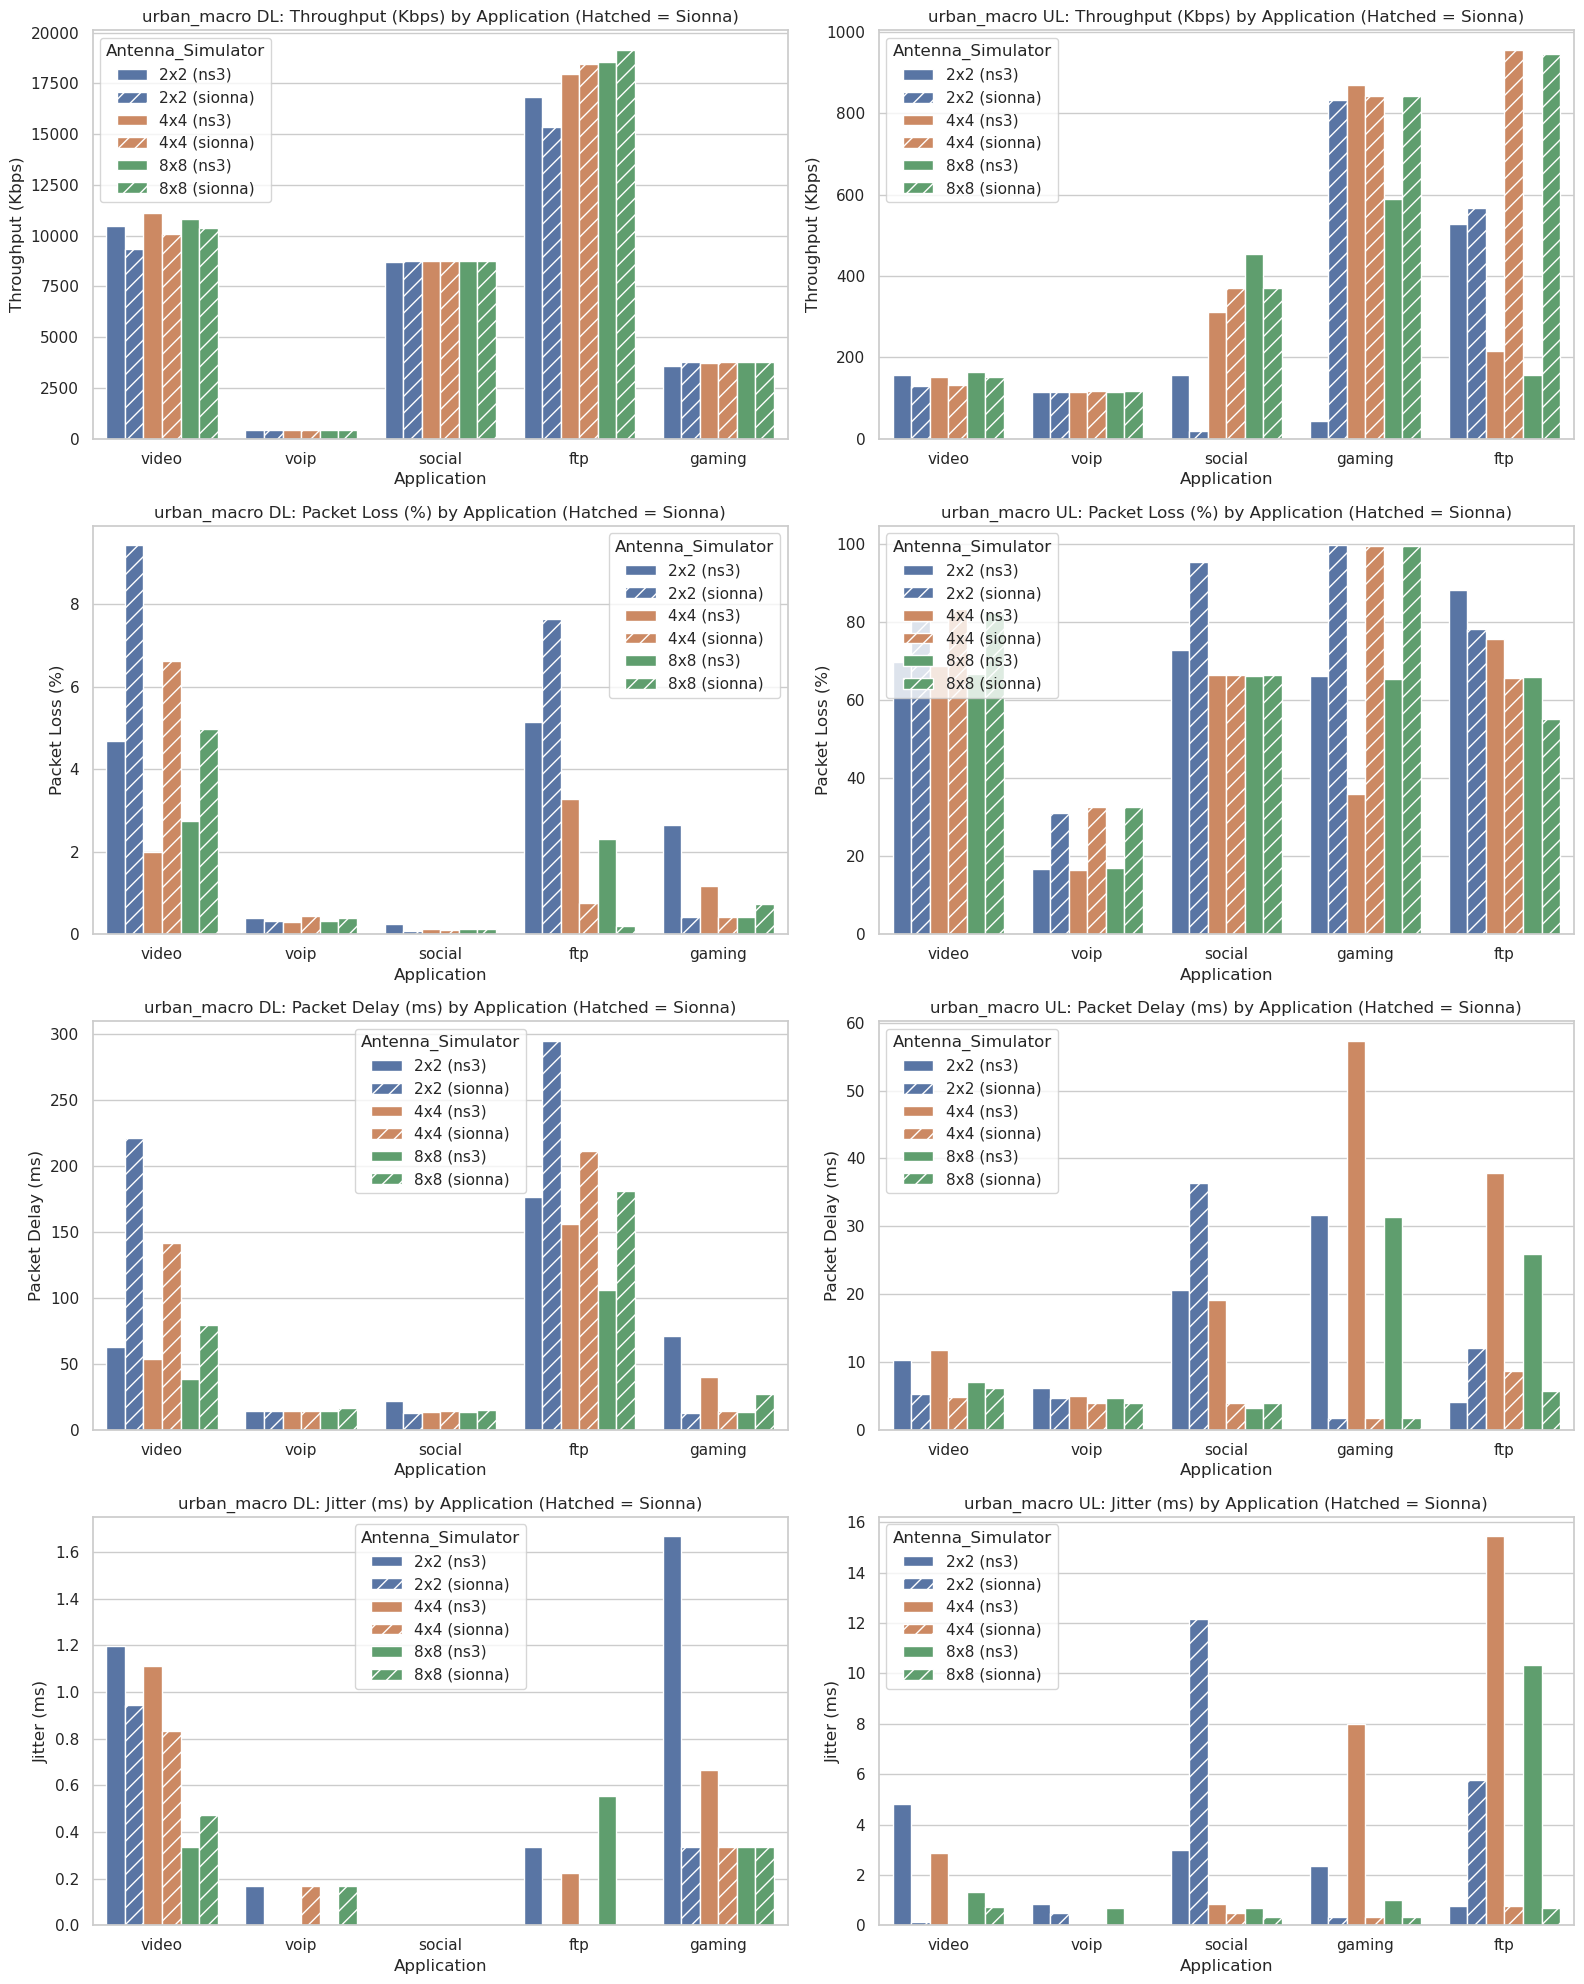
\includegraphics[width=\textwidth]{images/urban_macro_flow_metrics.png}
    \caption{Urban macro Application-related metrics by traffic type, direction, and
        gNB array size.}
    \label{fig:exp2-urban-macro-flow}
\end{figure*}


\subsubsection{Propagation-related Metrics}
\label{subsubsec:exp2-urban-macro-propagation}

The propagation-related results are presented in Figure \ref{fig:exp2-urban-macro-propagation}.
Path loss and received power remain consistent across all antenna size in both simulators at roughly $83.5$ dB and $-37.5$ dBm respectively.
Both ns-3 and Sionna RT achieve nearly identical values for propagation related metrics but differences can only be observed in path delay, CQI and MCS.
Ns-3 estimate a path delay of approximately $220$ ns while Sionna RT estimate higher delay around $360$ ns across all antenna configurations.
Higher delay in Sionna RT was due to taking into consideration for multipath components.

Similarly, lower CQI and MCS values are observed in Sionna RT than ns-3 for all antenna configurations.
For instance, in the $2 \times 2$ configuration, Sionna RT reports an average CQI of $9.5$ and MCS of $16.5$ while ns-3 estimates a CQI of $10.5$ and MCS of $17.5$.
Nevertheless, increasing gNB array size from $2 \times 2$ to $8 \times 8$ improves CQI and MCS in both simulators.
For example,  Sionna RT reports an average CQI of $10$ and MCS of $17$ at $8\times8$ configuration while ns-3 estimates a CQI of $11$ and MCS of $18$.
Improving CQI and MCS according to gNB array size validate that increasing the array size enhances beamforming capabilities and effectively reduces impact of environment and improves overall link quality.


\begin{figure*}[t]
    \centering
    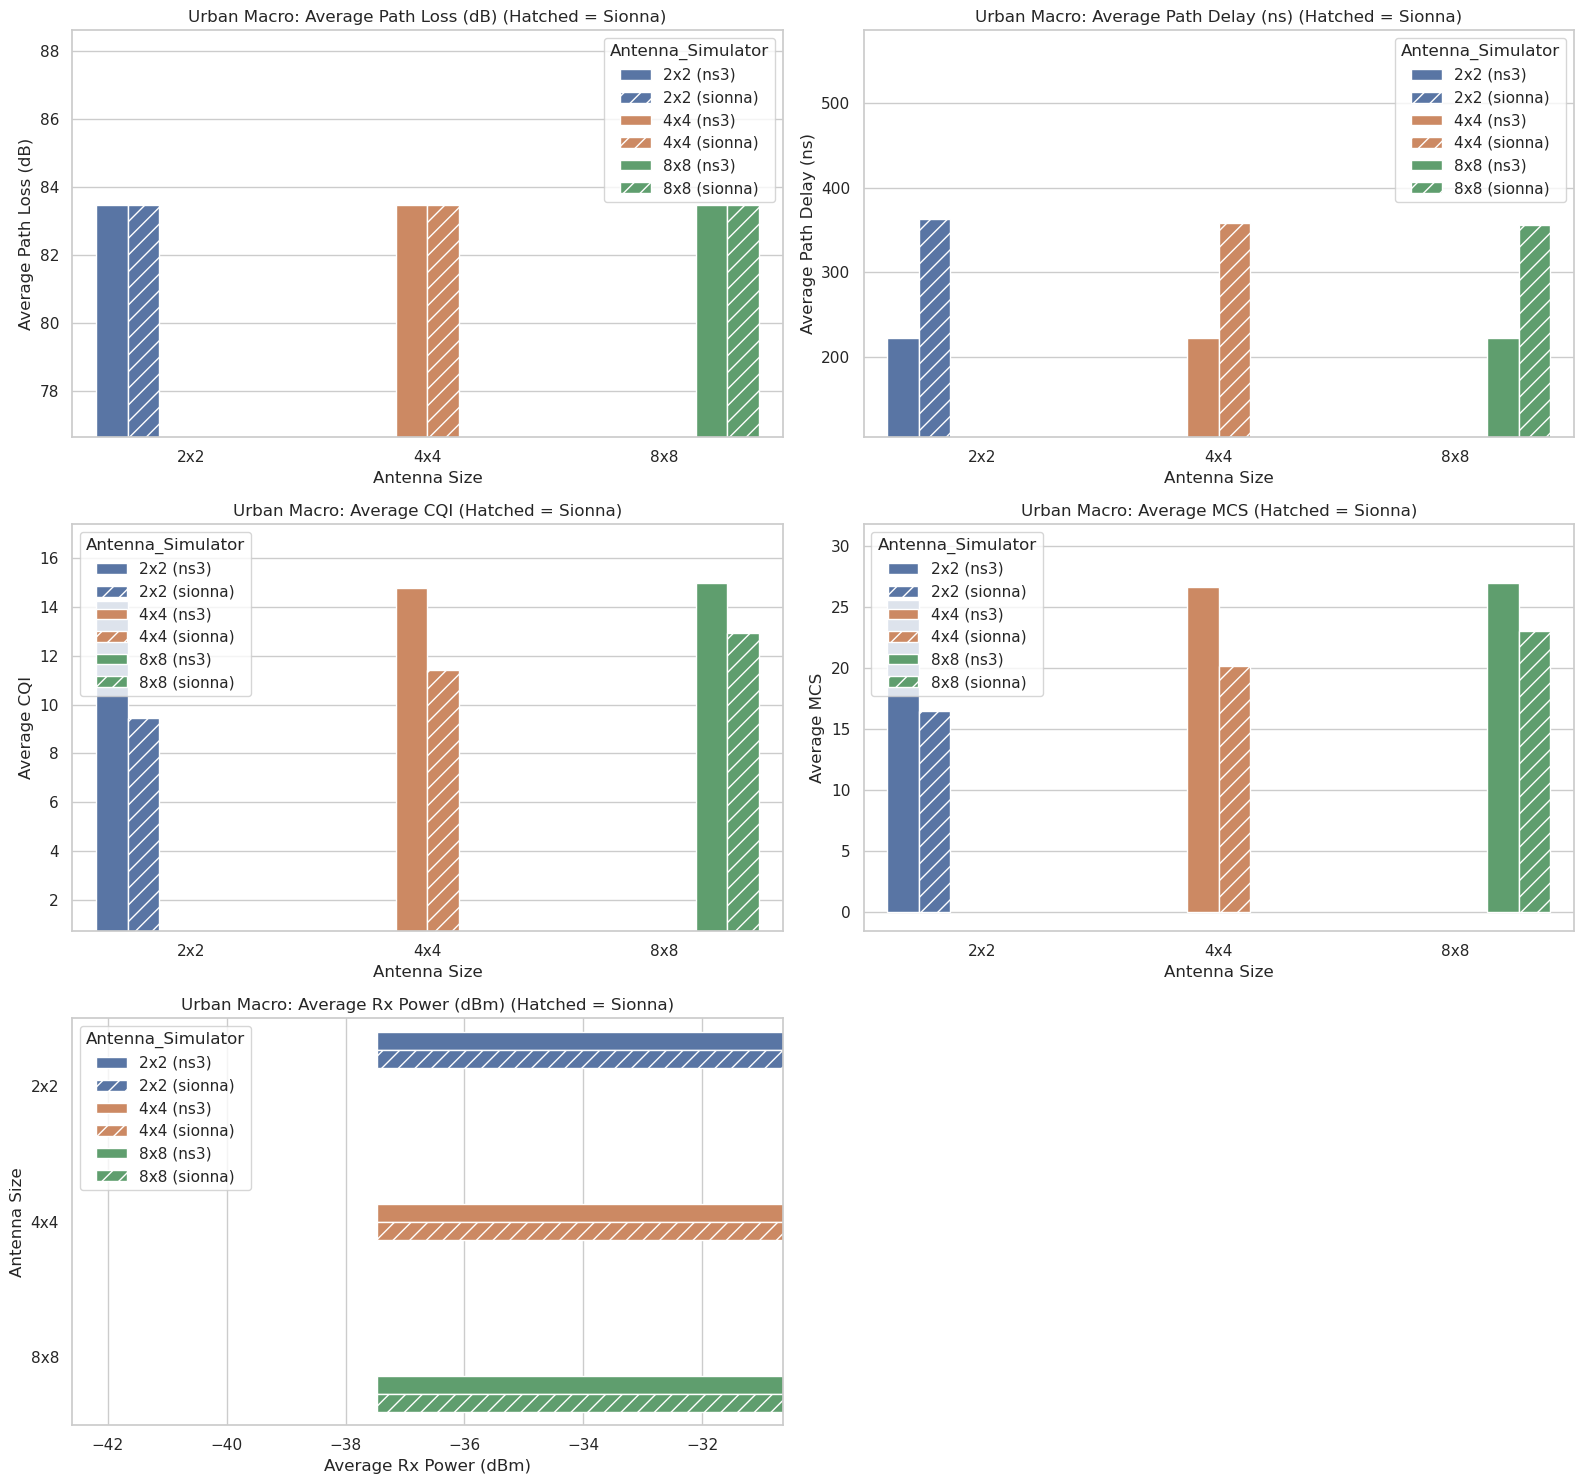
\includegraphics[width=\textwidth]{images/urban_macro_propagation_metrics.png}
    \caption{Urban macro propagation-related metrics by channel mode and gNB array
        size.}
    \label{fig:exp2-urban-macro-propagation}
\end{figure*}


\subsubsection{Energy Consumption-related Metrics}
\label{subsubsec:exp2-urban-macro-energy}\

In Figure \ref{fig:exp2-urban-macro-energy}, the energy consumptions of gNB and UEs by array size, and traffic load are presented.
The power consumption of gNB scales accordingly with both antenna array size and traffic load and both simulators show similar scaling trends.
For instance, both ns-3 and Sionna RT reports approximately $25$ W, $40$ W and $100$ W for $2\times2, 4\times4, 8\times8$ array configurations under low traffic load.
However, Sionna RT reports slightly higher power consumption than ns-3 for all antenna configurations.
The reason is link to lower CQI and MCS values estimated by Sionna RT, which alters resource block allocations and transmission durations compared to ns-3.
These results show that increasing gNB array size improve performance but at the cost of significantly higher energy consumption.

The power consumption of UE remains relatively stable for all antenna configurations in both simulators but scale noticeably with traffic load.
The UE power consumption increases from approximately $0.058$ W at low load to nearly $0.095$ W at high load.
Both simulator observe nearly identical UE power consumption across all configurations but Sionna RT consumes slightly higher energy than ns-3.
This is because UE are constrained to $2 \times 2$ antenna configuration in this experiment.

\begin{figure*}[t]
    \centering
    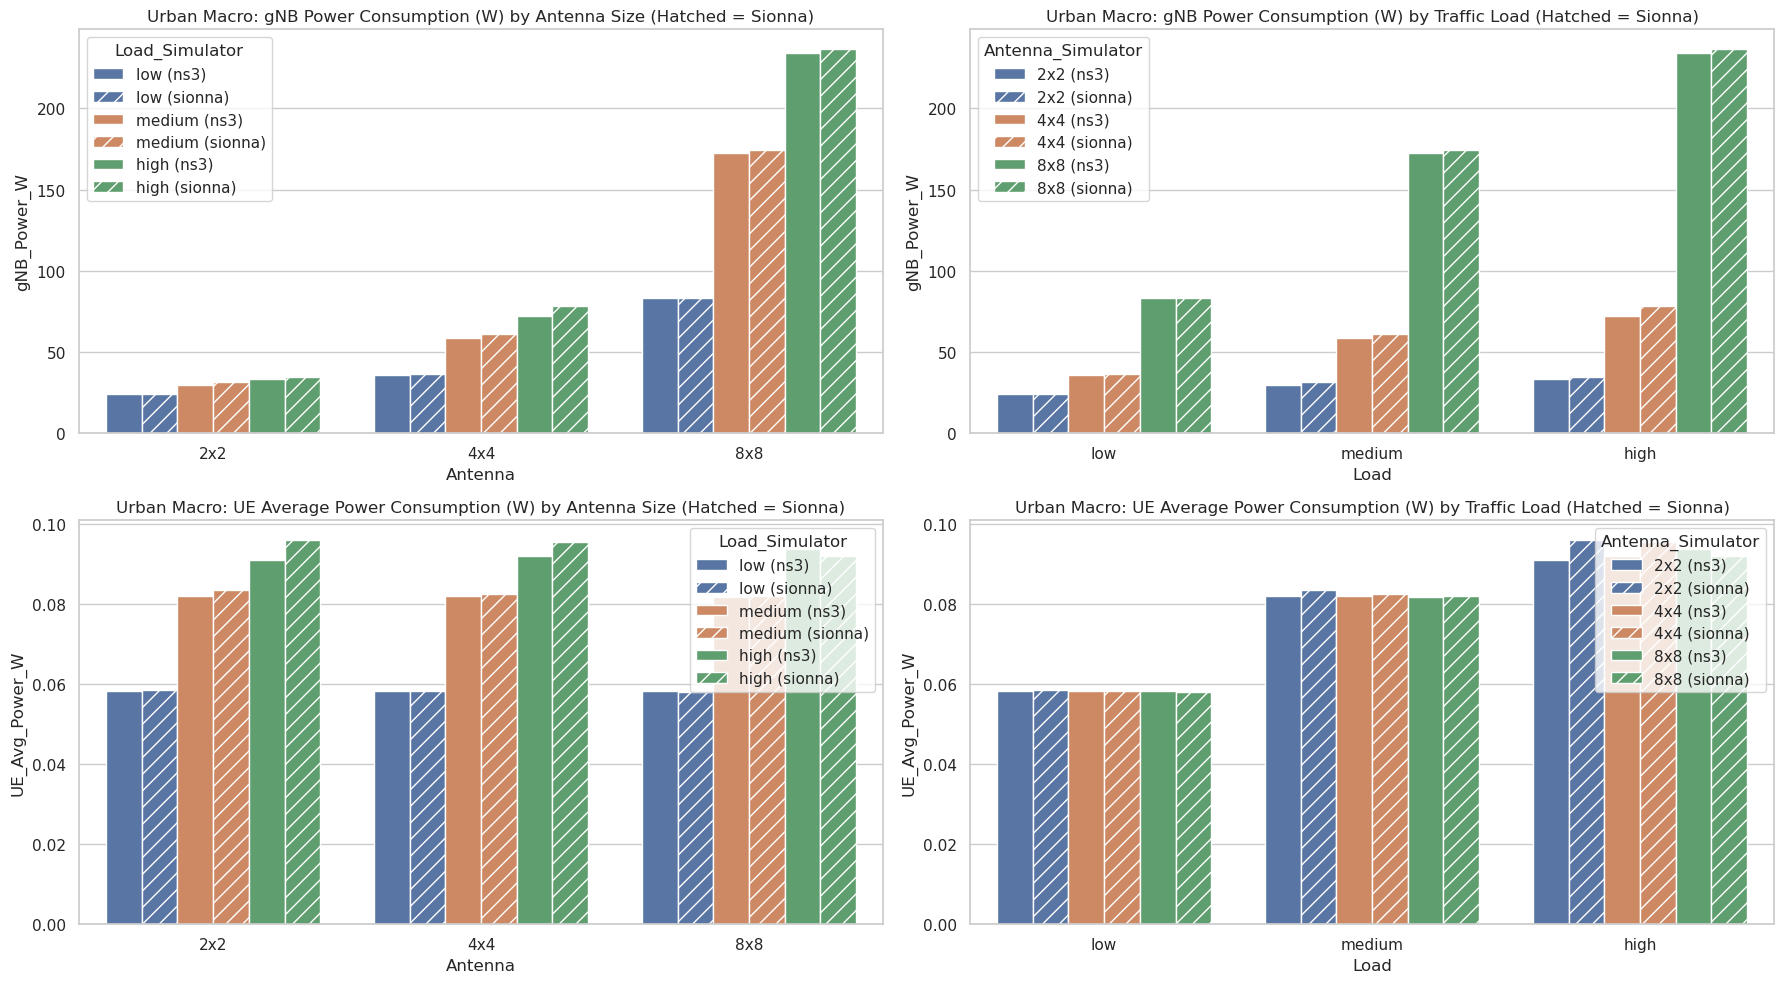
\includegraphics[width=\textwidth]{images/urban_macro_power_consumption.png}
    \caption{Urban macro energy consumptions of gNB and UEs by array size, and
        traffic load.}
    \label{fig:exp2-urban-macro-energy}
\end{figure*}

\subsection{Urban Micro Scenario}
\label{subsec:exp2-urban-micro}

The urban micro scenario is designed to simulate the dense street-level environment where gNB is deployed at lower elevation of $10$ m, typically below the surrounding rooftops.
In this scenario, the likelihood of non-line-of-sight (NLOS) conditions and strong multipath effects due to scattering from nearby buildings and street furniture is higher compared to the macro scenario.
The complex propagation environment presents unique challenges for establishing reliable links, especially for high-throughput applications.

\subsubsection{Application-related Metrics}
\label{subsubsec:exp2-urban-micro-flow}

Figure \ref{fig:exp2-urban-micro-flow} illustrates the application-level flow metrics for the urban scenario.
A comparative analysis between the statistical ns-3 model (solid bars) and the ray-tracing Sionna model (hatched bars) reveals substantial differences in how each simulator resolves the complex 3D urban environment.
In terms of downlink throughput, Sionna RT consistently achieve higher throughput for data-intensive applications such as FTP and gaming compared to ns-3.
For example, in Sionna RT, FTP throughput reach nearly $20$ Mbps with $4 \times 4$ and $8 \times 8$ gNB antenna array sizes while ns-3 reach around $15$ Mbps.
This mean that Sionna RT approach capture multipath components (reflections and diffractions) from urban structures which lead to higher downlink throughput than ns-3 approach when MIMO spatial multiplexing is leveraged.
Consistent with the trends observed in the macro scenario (Section~\ref{subsec:exp2-urban-macro}), scaling from $2\times2$ to $8\times8$ clearly improves throughput in both simulators.

The packet loss metrics further emphasize the environmental impact.
In downlink, ns-3 get high packet loss for FTP and gaming, nearly $30\%$ in $2\times2$ configuration, while Sionna RT get lower loss rate for these applications.
In contrast, Sionna~RT reports higher loss for video traffic at $2\times2$.
In both cases, scaling to $8\times8$ reduces downlink packet loss to near-zero for most applications, demonstrating how massive MIMO overcomes urban blockage.
The uplink remains severely loss-limited ($60\%$–$90\%$ in both simulators), reflecting the fundamental constraint that UE transmit power is insufficient to overcome dense urban obstacles without a reciprocal beamforming advantage at the receiver.

Packet delay and jitter metrics also align with the previous observations.
Downlink delay is worst under $2 \times 2$ array configuration, with ns-3 experiencing extreme spikes for FTP $>350$ ms and Sionna RT showing elevated delays for video and social traffic.
The multipath components captured by ray-tracing can introduce variable signal arrival times, occasionally increasing delay and jitter for continuous streams in Sionna RT.
However, as the gNB array scales to $8 \times 8$, both delay and jitter drop significantly which confirms that massive MIMO is essential for meeting the strict latency and reliability requirements of 6G applications in dense urban areas.


\begin{figure*}[t]
    \centering
    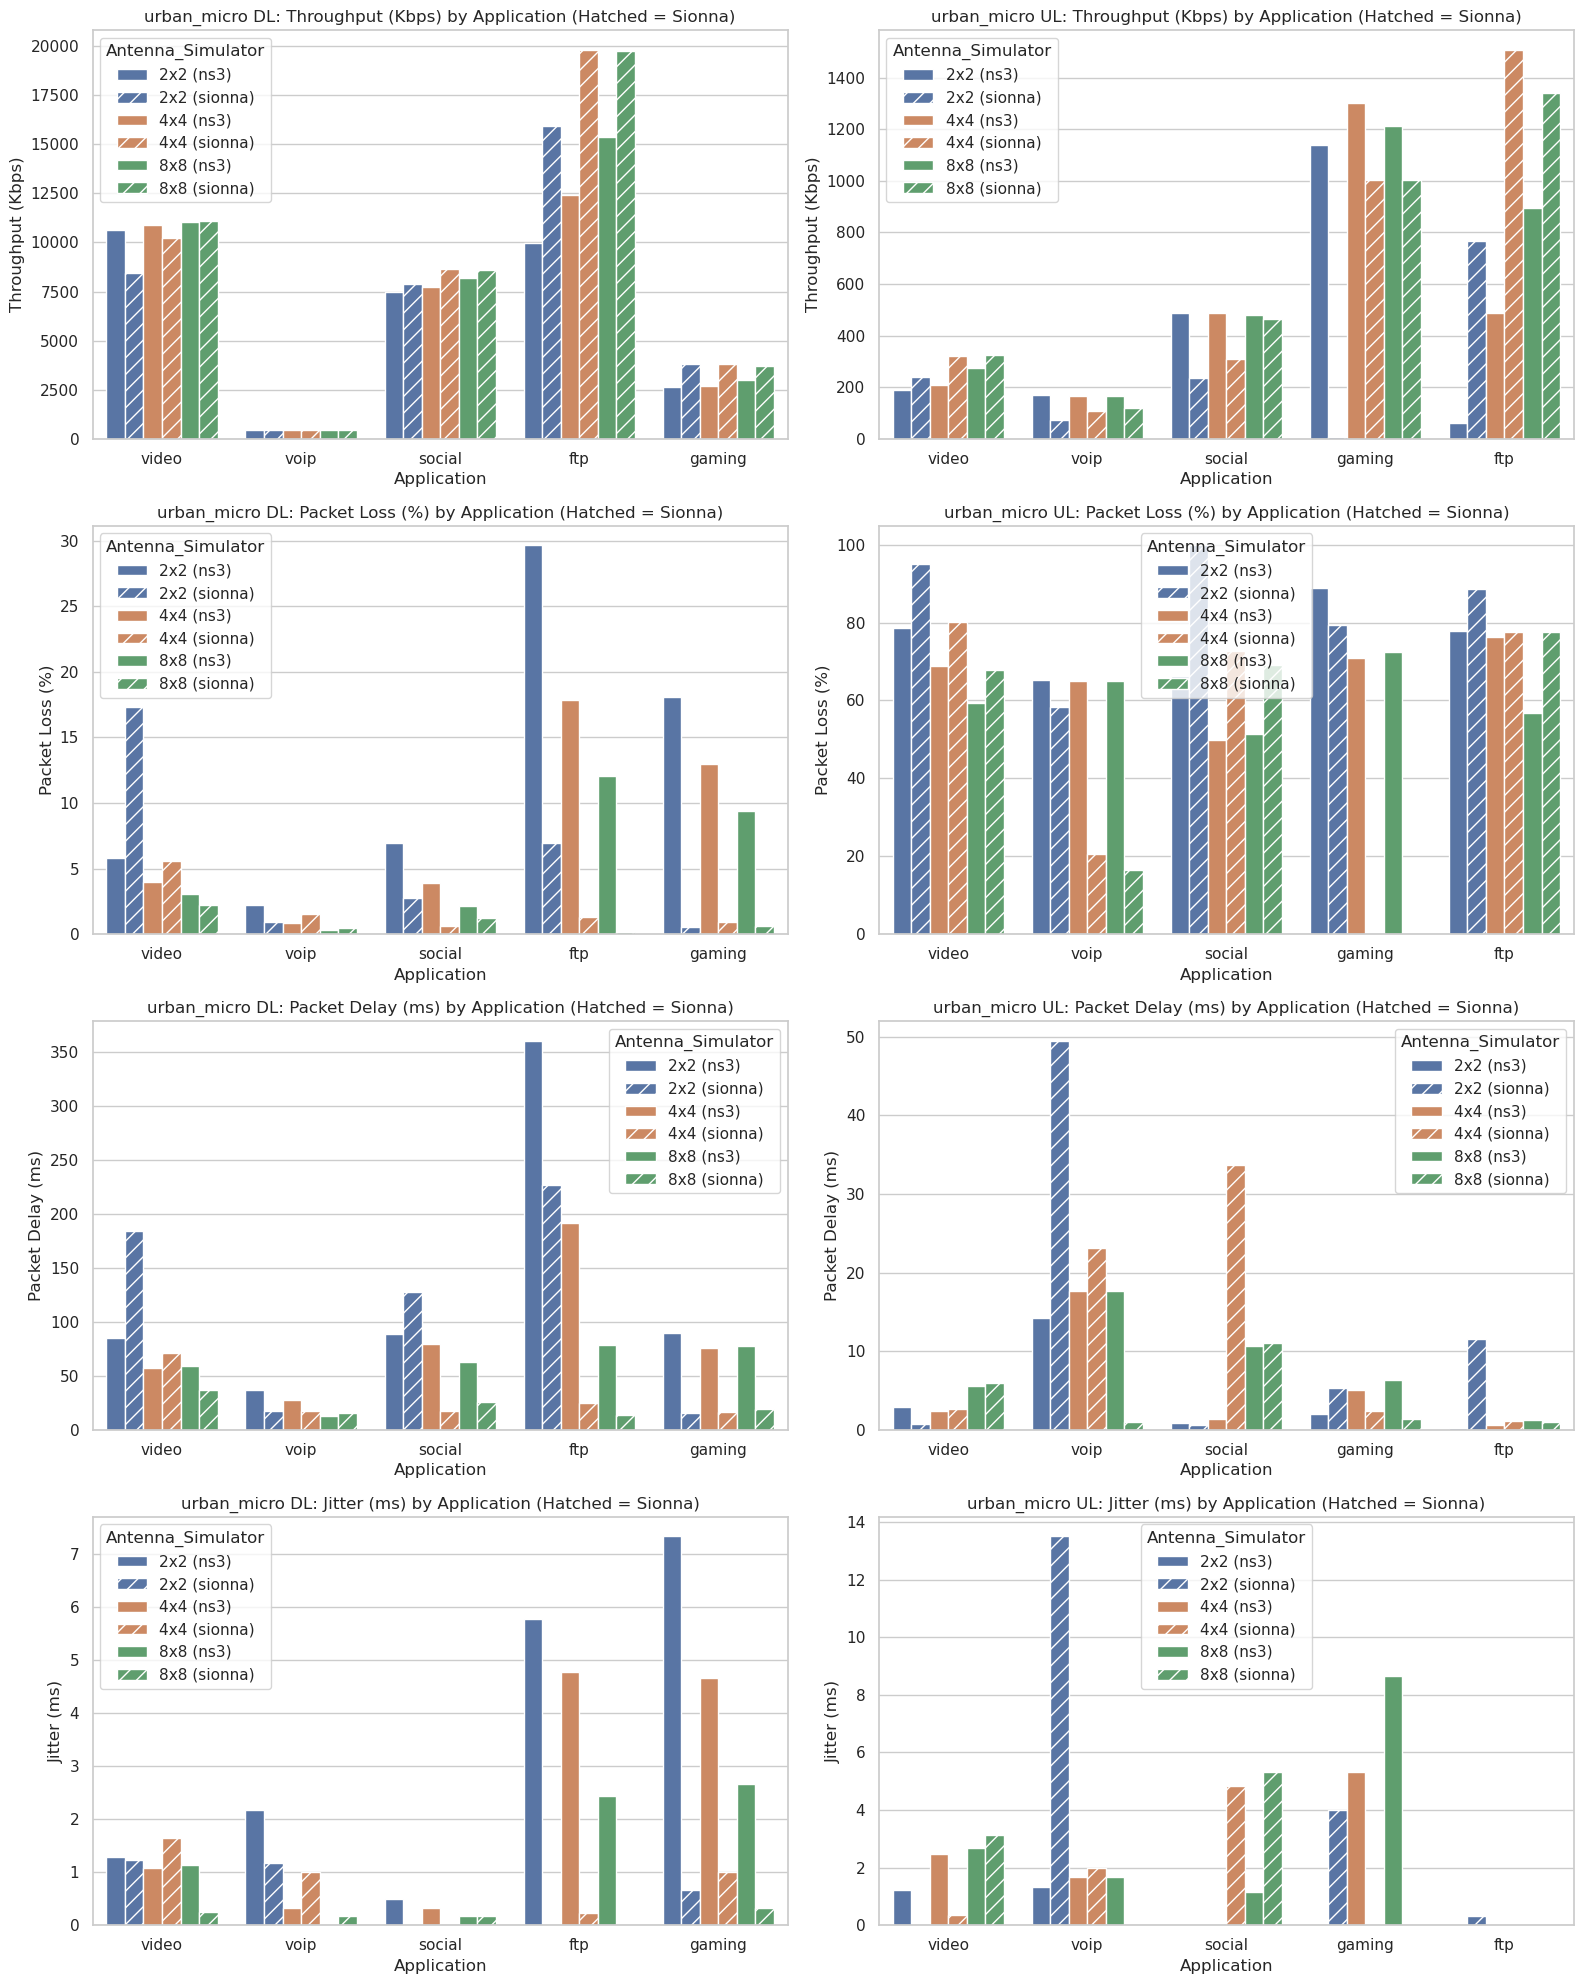
\includegraphics[width=\textwidth]{images/urban_micro_flow_metrics.png}
    \caption{Urban micro Application-related metrics by traffic type, direction, and gNB array size.}
    \label{fig:exp2-urban-micro-flow}
\end{figure*}


\subsubsection{Propagation-related Metrics}
\label{subsubsec:exp2-urban-micro-propagation}

The propagation-related results are presented in Figure \ref{fig:exp2-urban-micro-propagation}.
Average path loss, received power remain consistent across all antenna size at roughly $95.5$ dB and $-62.5$ dBm for both simulators.
Both ns-3 and Sionna RT report nearly identical values for propagation related metrics.

The simulators diverge on path delay and channel quality metrics.
As in the macro scenario (Section~\ref{subsec:exp2-urban-macro}), Sionna~RT reports a higher mean path delay ($178$~ns vs.\ $120$~ns for ns-3), consistent with its multipath-aware propagation accounting over the dense street-level geometry.

Similarly, Sionna RT predicts lower average CQI and MCS values compared to ns-3.
For instance, in the $2 \times 2$ configuration, Sionna RT reports an average CQI of $6$ and MCS of $10$ while ns-3 estimates a CQI of $9.5$ and MCS of $16.5$.
The lower CQI and MCS values in Sionna RT highlight the impact of the detailed multipath fading and interference captured by the ray tracer, leading to a harsher but more realistic channel quality assessment.
Nevertheless, as the antenna array size scales from $2 \times 2$ to $8 \times 8$, both CQI and MCS improve significantly in both simulators.
This further confirms that larger arrays are essential for overcoming the harsh mmWave urban channel.


\begin{figure*}[t]
    \centering
    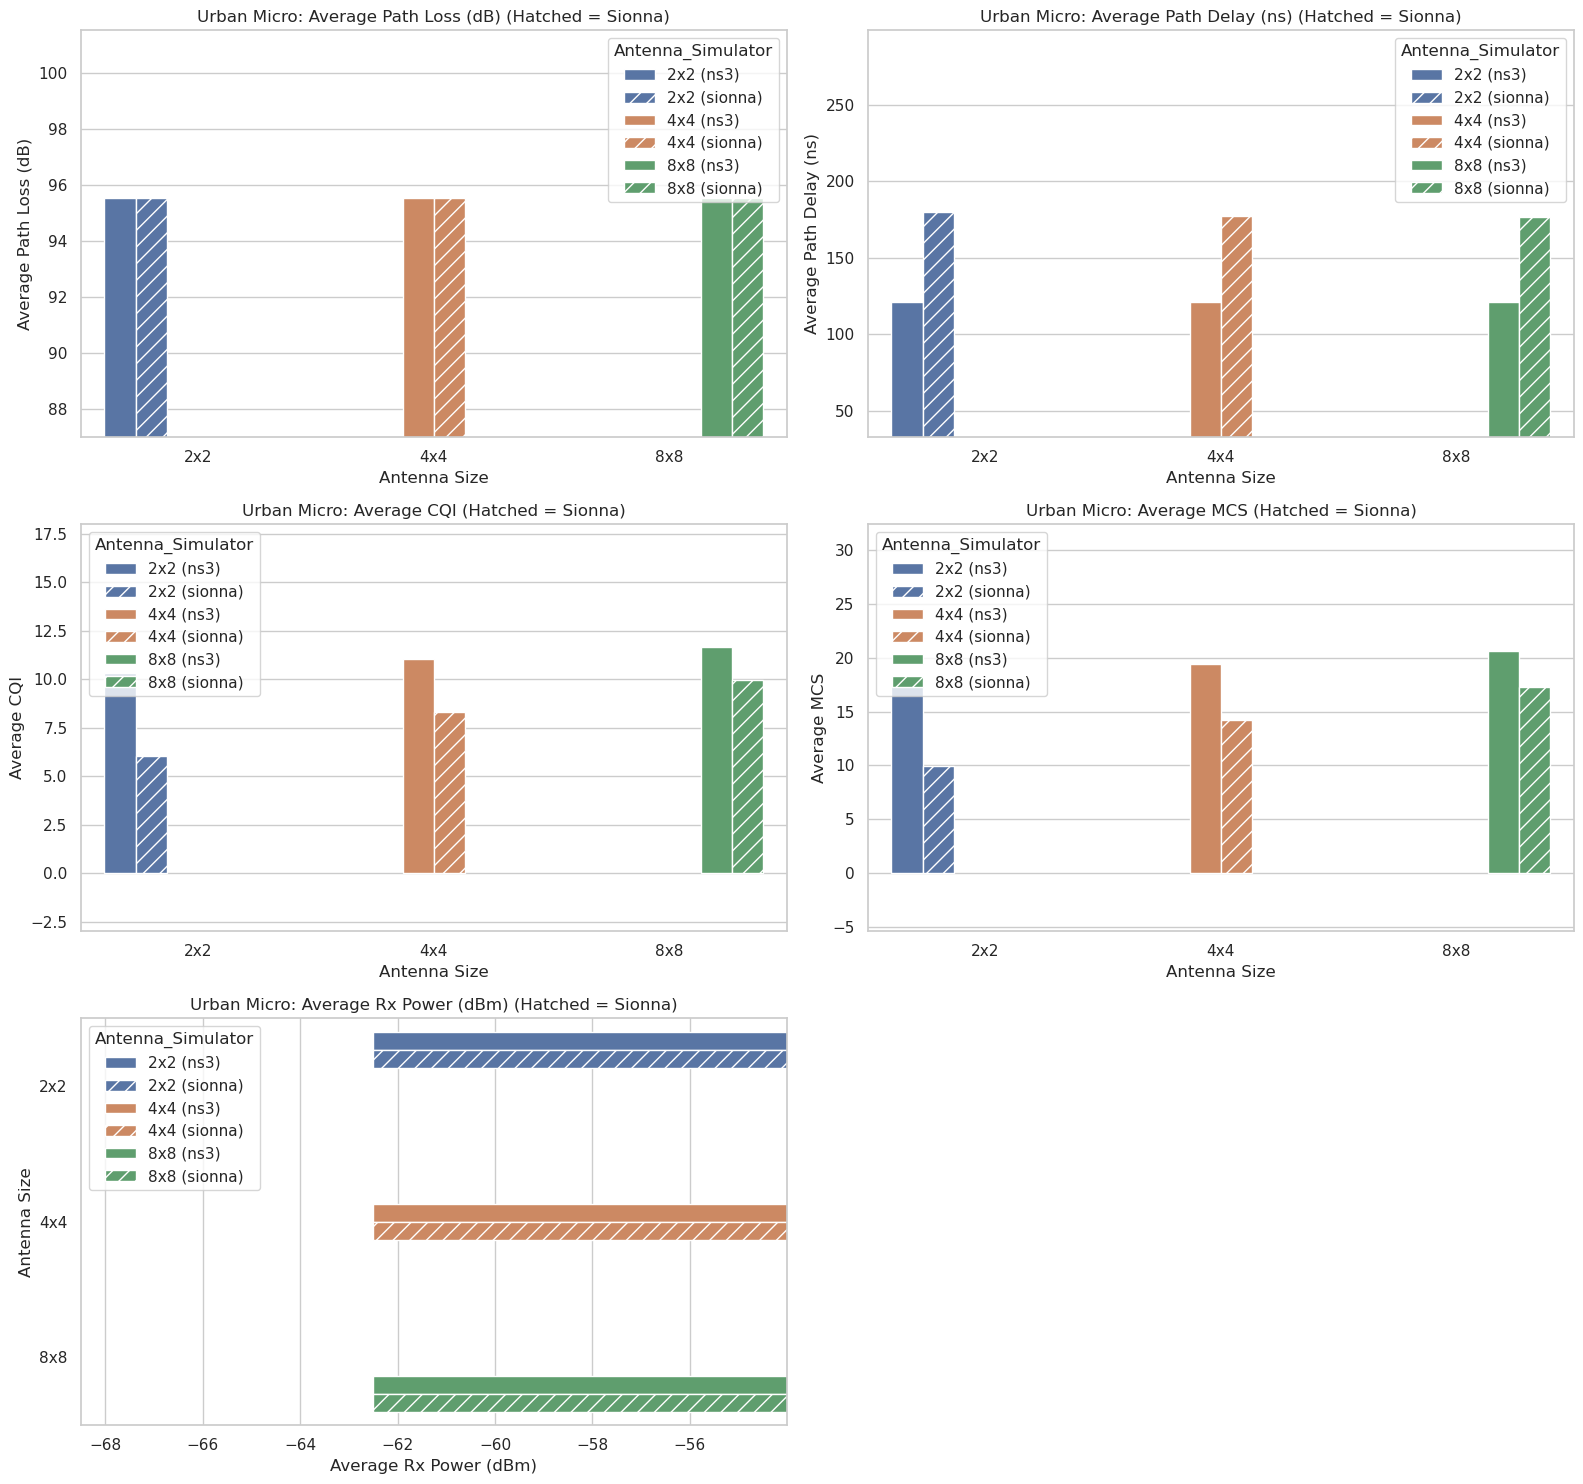
\includegraphics[width=\textwidth]{images/urban_micro_propagation_metrics.png}
    \caption{Urban micro propagation-related metrics by channel mode and gNB array size.}
    \label{fig:exp2-urban-micro-propagation}
\end{figure*}


\subsubsection{Energy Consumption-related Metrics}
\label{subsubsec:exp2-urban-micro-energy}

In Figure \ref{fig:exp2-urban-micro-energy}, the energy consumptions of gNB and UEs by array size, and traffic load are presented.
The gNB energy scaling pattern mirrors the macro scenario: power increases with both array size and traffic load, and Sionna~RT reports slightly lower consumption than ns-3 under high load due to its lower CQI/MCS estimates altering resource allocation.
Under low load, both simulators report $23$~W, $33$~W, and $68$~W for $2\times2$, $4\times4$, and $8\times8$ respectively.
The urban micro scenario adds a notable high-load extreme: the $8\times8$ configuration reaches $215$~W (ns-3) and $193$~W (Sionna~RT) — roughly three times the macro high-load figure — driven by the combined demand of a 400~MHz mmWave channel and dense multipath-induced retransmissions.

UE power consumption ($0.05$~W at low load, $0.09$~W at high load) is nearly identical between the two simulators and independent of gNB array size, confirming that UEs are operating at near-maximum transmit power against the challenging urban channel regardless of the gNB configuration.

\begin{figure*}[t]
    \centering
    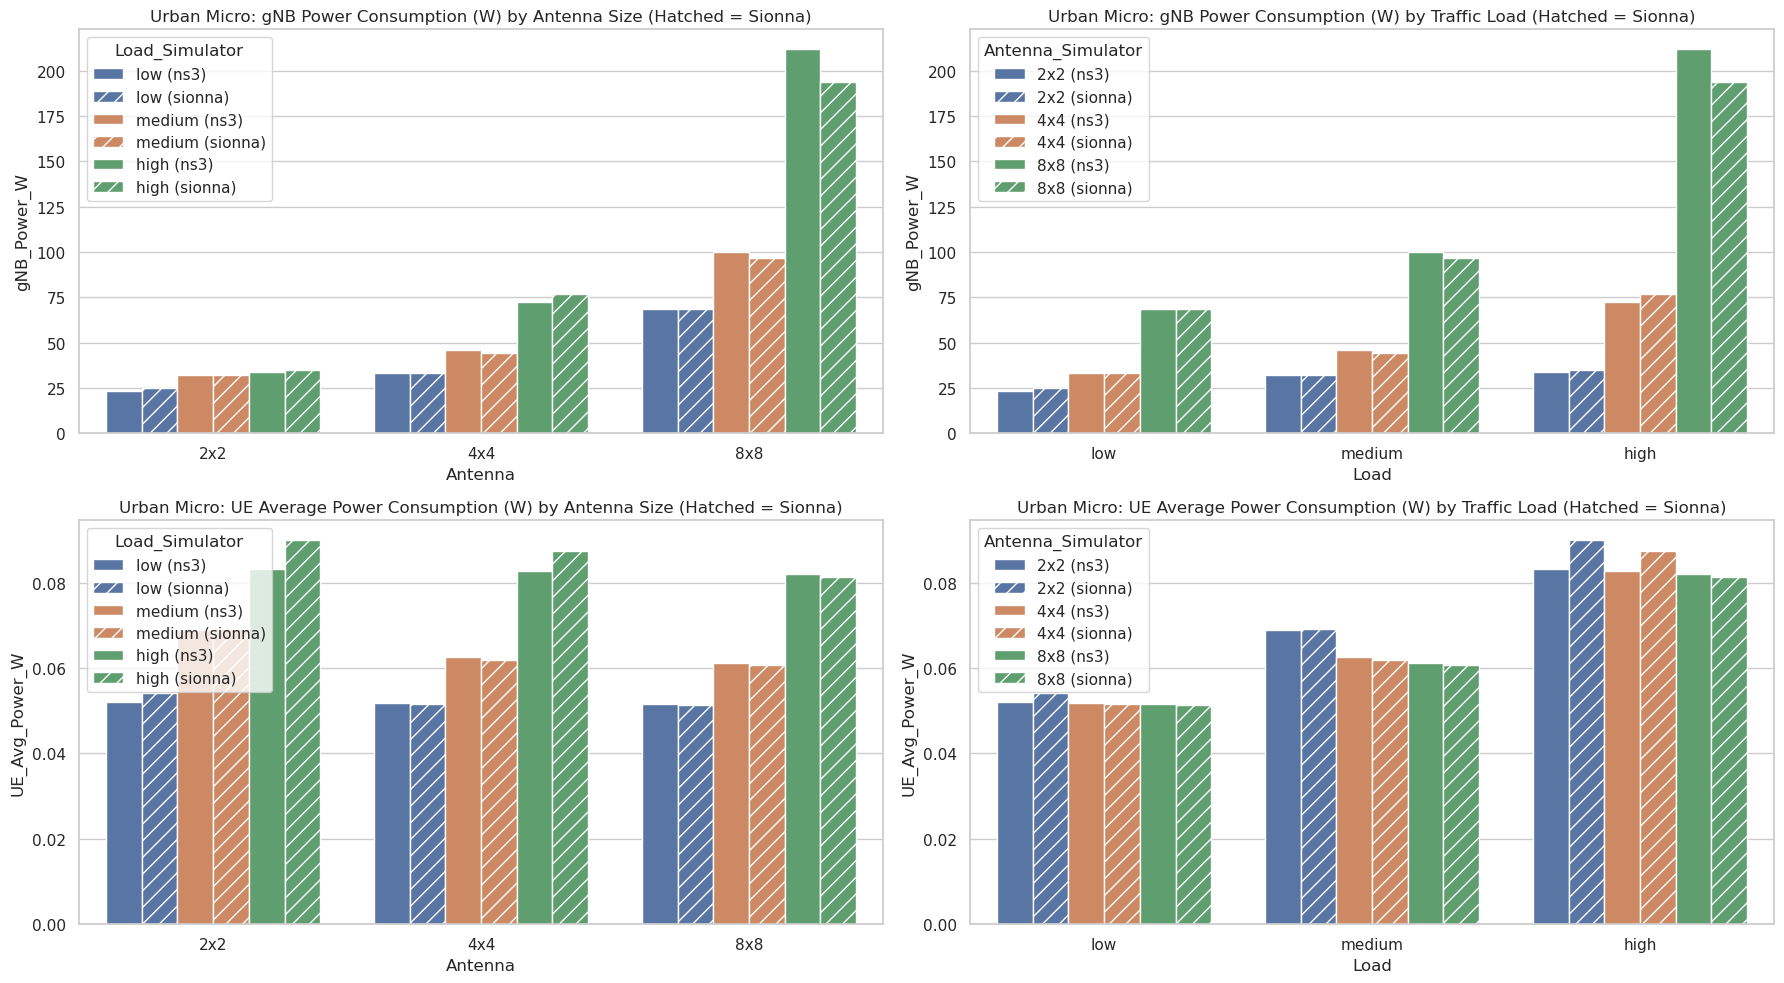
\includegraphics[width=\textwidth]{images/urban_micro_power_consumption.png}
    \caption{Urban micro energy consumptions of gNB and UEs by array size, and traffic load.}
    \label{fig:exp2-urban-micro-energy}
\end{figure*}


\begin{figure*}[t]
    \centering
    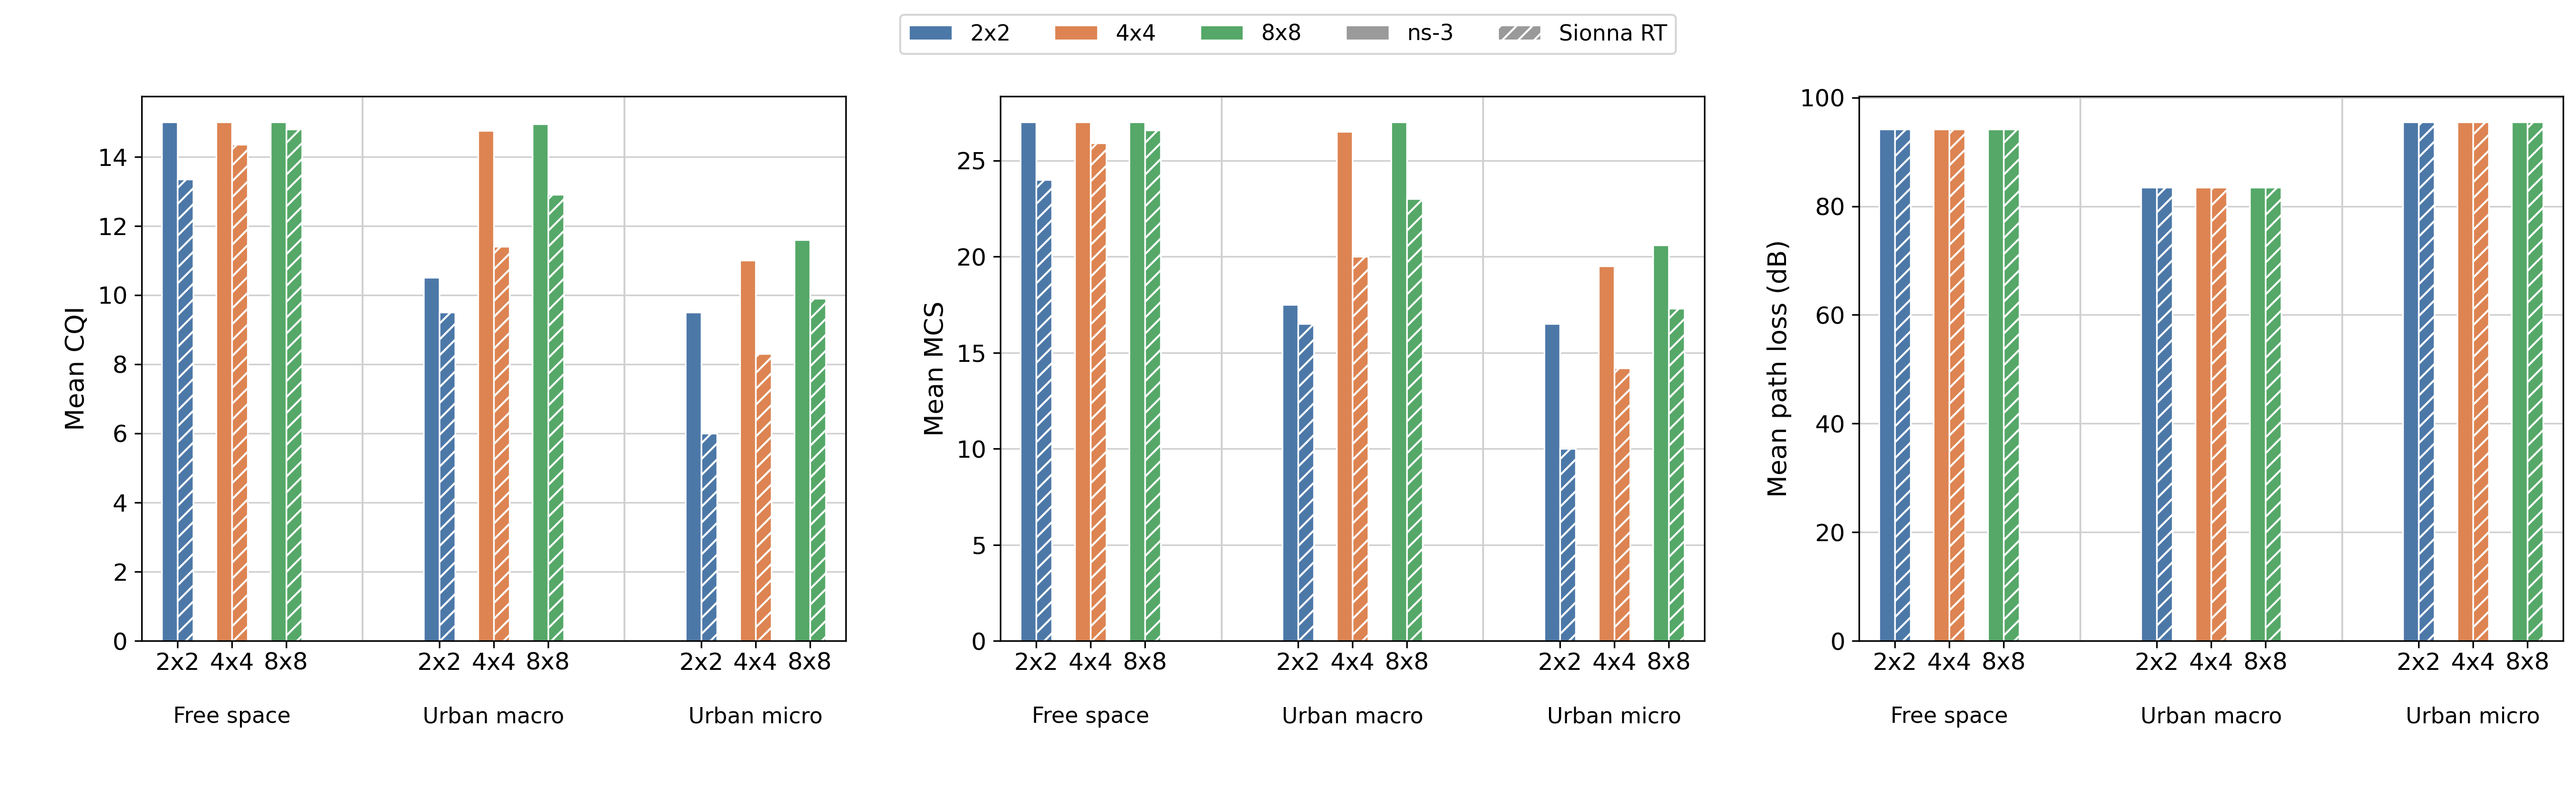
\includegraphics[width=\textwidth]{images/channel_quality_comparison.png}
    \caption{Propagation-related metrics (path loss, received power, path delay, CQI, MCS) across three radio environments and gNB array sizes, comparing ns-3 and Sionna~RT under high traffic load.}
    \label{fig:exp2-channel-quality}
\end{figure*}

\begin{figure*}[t]
    \centering
    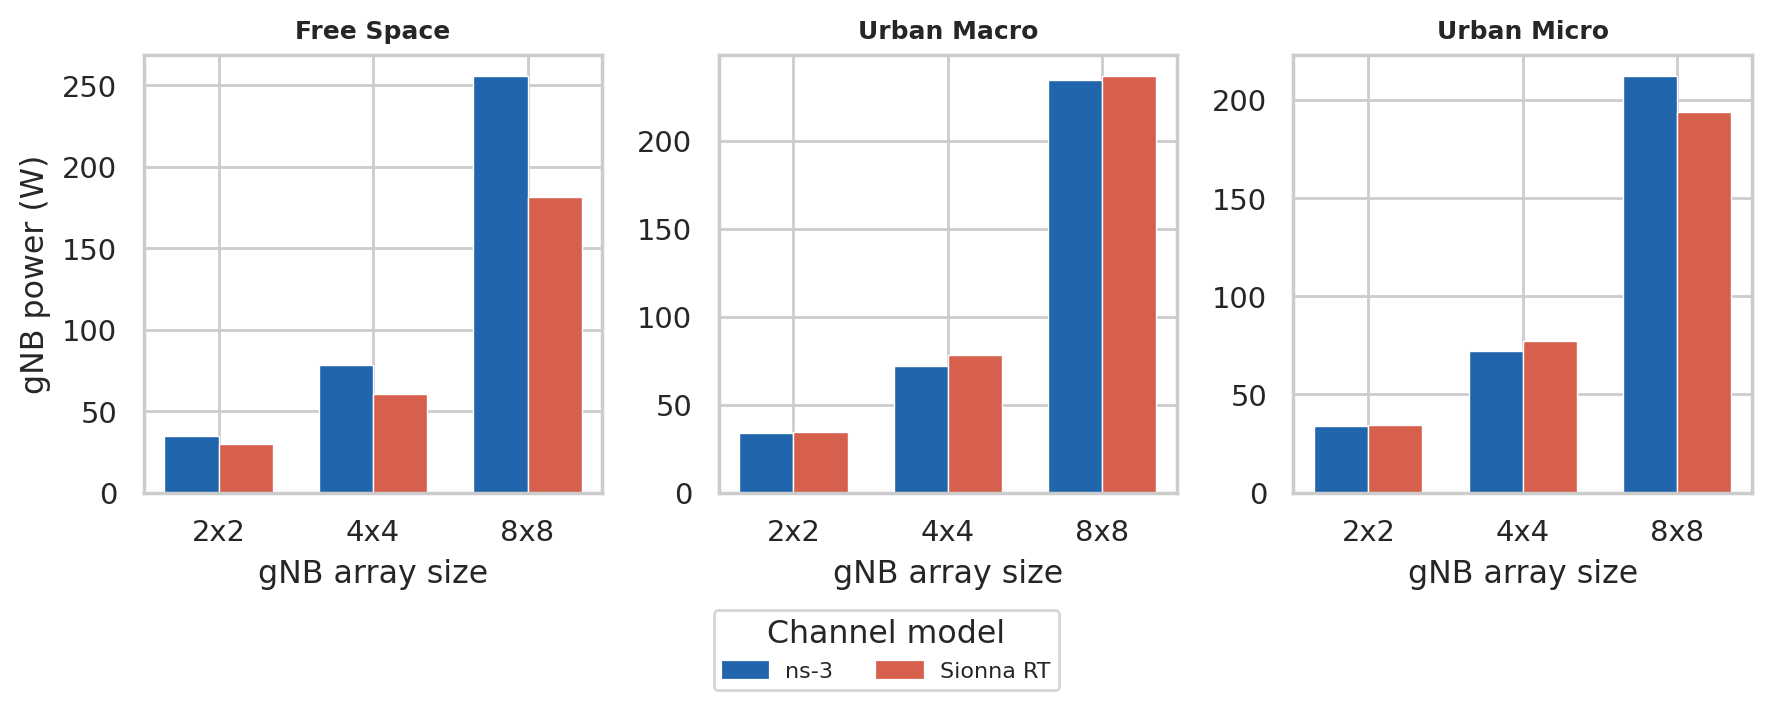
\includegraphics[width=\textwidth]{images/gnb_power_comparison.png}
    \caption{gNB power consumption (W) by array size and radio environment, comparing ns-3 and Sionna~RT under high traffic load.}
    \label{fig:exp2-gnb-power}
\end{figure*}
